\documentclass[9pt,aspectratio=169,xcolor=table]{beamer}

%~~~~~~~~~~~~~~~~~~~~~~~~~~~~~~~~~~~~~~~~~~~~~~~~~~~~~~~~~~~~~~~~~~~~~~~~~~~~~~
% Use roboto Font (recommended)
\usepackage[sfdefault]{roboto}
\usepackage[utf8]{inputenc}
\usepackage[T1]{fontenc}
%~~~~~~~~~~~~~~~~~~~~~~~~~~~~~~~~~~~~~~~~~~~~~~~~~~~~~~~~~~~~~~~~~~~~~~~~~~~~~~

%~~~~~~~~~~~~~~~~~~~~~~~~~~~~~~~~~~~~~~~~~~~~~~~~~~~~~~~~~~~~~~~~~~~~~~~~~~~~~~
% Define where theme files are located. ('/styles')
\usepackage{styles/fluxmacros}
\usefolder{styles}
% Use Flux theme v0.1 beta
% Available style: asphalt, blue, red, green, gray
\usetheme[style=hunter]{flux}
%~~~~~~~~~~~~~~~~~~~~~~~~~~~~~~~~~~~~~~~~~~~~~~~~~~~~~~~~~~~~~~~~~~~~~~~~~~~~~~

%~~~~~~~~~~~~~~~~~~~~~~~~~~~~~~~~~~~~~~~~~~~~~~~~~~~~~~~~~~~~~~~~~~~~~~~~~~~~~~
% Extra packages
\usepackage{booktabs}
\usepackage{colortbl}
\usepackage{ragged2e}
\usepackage{amssymb}
\usepackage{multirow}
\usepackage{tikz}
\usetikzlibrary{arrows.meta, positioning, fit, backgrounds, calc, decorations.pathreplacing}
\setbeamertemplate{itemize items}[square]
\usepackage[scaled=.8]{beramono}
\usepackage{listings}
\usepackage{styles/lstlangarm}
\usepackage{array}
\definecolor{bgcolor}{HTML}{F2E9E9}
% lstlangarm.sty references \color{mauve} for string literals but never defines
% it -- only fires when a listing contains a string. Define it here.
\definecolor{mauve}{rgb}{0.58,0,0.82}
% lstlangarm's C style sets commentstyle=green!20, which is unreadable on the
% pink listing background. Darken it globally.
\lstset{commentstyle=\color{green!45!black}}
% ragged-right fixed-width column -- must be defined in the preamble, never
% inside a frame (\newcolumntype's #1 breaks beamer's frame scanner)
\newcolumntype{R}[1]{>{\RaggedRight\arraybackslash}p{#1}}
%~~~~~~~~~~~~~~~~~~~~~~~~~~~~~~~~~~~~~~~~~~~~~~~~~~~~~~~~~~~~~~~~~~~~~~~~~~~~~~
% Table striping: odd rows white, even rows very light gray.
% Needs \documentclass[...,xcolor=table]{beamer} (beamer loads xcolor itself,
% so the option must go on the class, not \usepackage).
\definecolor{stripe}{gray}{0.94}
% \striped makes body rows alternate white, gray, white, ... starting white.
% \rowcolors counts from the first coloured body row; the header is not counted.
\newcommand{\striped}{\rowcolors{1}{white}{stripe}}
%~~~~~~~~~~~~~~~~~~~~~~~~~~~~~~~~~~~~~~~~~~~~~~~~~~~~~~~~~~~~~~~~~~~~~~~~~~~~~~

%~~~~~~~~~~~~~~~~~~~~~~~~~~~~~~~~~~~~~~~~~~~~~~~~~~~~~~~~~~~~~~~~~~~~~~~~~~~~~~
% TikZ block styles -- matches ch1/ch2
% Colour variables are named identically in the book's stm32primer.tex, so any
% tikzpicture using only the \tikzset{...} styles below can be copied verbatim
% between slides and book. Only the \definecolor/\colorlet VALUES differ: the
% book is printed, so it keeps every stroke pure black with muted fills. These
% slides are projected, so both fill AND stroke are bright and saturated to
% grab attention -- see stm32primer.tex for the print palette.
\definecolor{blkfill}{HTML}{DDEEDD}
\definecolor{blkline}{HTML}{355E3B}
\definecolor{accentfill}{HTML}{FFE0B2}
\definecolor{accentline}{HTML}{E65100}
\definecolor{memfill}{HTML}{DFF5DA}
\definecolor{memline}{HTML}{2E7D32}
\definecolor{cellfill}{HTML}{FFFFFF}
\definecolor{cellline}{HTML}{424242}
\definecolor{bitmaskfill}{HTML}{DCEBFF}
\definecolor{bitmaskline}{HTML}{1565C0}
\definecolor{bithitfill}{HTML}{FFE0B2}
\definecolor{bithitline}{HTML}{E65100}
\tikzset{
  blk/.style   = {rectangle, rounded corners=2pt, draw=blkline, fill=blkfill,
                  thick, align=center, font=\small, minimum height=9mm, inner sep=3pt},
  cpublk/.style= {rectangle, rounded corners=2pt, draw=accentline, fill=accentfill,
                  thick, align=center, font=\small\bfseries, minimum height=9mm, inner sep=3pt},
  memblk/.style= {rectangle, rounded corners=2pt, draw=memline, fill=memfill,
                  thick, align=center, font=\small, minimum height=9mm, inner sep=3pt},
  cell/.style  = {rectangle, draw=cellline, fill=cellfill, align=center,
                  font=\small\ttfamily, minimum height=7mm, inner sep=2pt},
  bitcell/.style={rectangle, draw=cellline, fill=cellfill, thick,
                  minimum width=5.4mm, minimum height=5.4mm, inner sep=0pt,
                  font=\scriptsize\ttfamily, anchor=center},
  bitmask/.style={bitcell, fill=bitmaskfill, draw=bitmaskline},
  bithit/.style ={bitcell, fill=bithitfill, draw=bithitline, font=\scriptsize\ttfamily\bfseries},
  rowlab/.style ={font=\scriptsize, text=Gray, anchor=east},
  oplab/.style  ={font=\scriptsize\itshape, text=Gray, anchor=west},
  lbl/.style   = {font=\scriptsize, text=Gray},
  flow/.style  = {-{Stealth[length=2mm]}, thick, draw=blkline},
  busline/.style={thick, draw=cellline},
}
% NOTE (theme quirks -- all fail SILENTLY, always page through the PDF):
%  - a second \\ inside a nested {...} group in a TikZ node breaks parsing
%  - {\small ...} wrapped around a nested itemize eats the frame title + list
%  - \usebeamercolor on a [plain] frame falls through to an unstyled default
%  - \newcolumntype inside a frame breaks beamer's frame scanner
%  - lstlisting needs \begin{frame}[fragile]
%  - a TikZ picture wider than its column silently overflows into neighbours
%~~~~~~~~~~~~~~~~~~~~~~~~~~~~~~~~~~~~~~~~~~~~~~~~~~~~~~~~~~~~~~~~~~~~~~~~~~~~~~

%%%%%%%%%%%%%%%%%%%%%%%%%%%%%%%%%%%
%% BEGIN CONDITIONAL COMPILATION %%
%%%%%%%%%%%%%%%%%%%%%%%%%%%%%%%%%%%
\newif\ifwebex
%\webextrue % uncomment to generate section separator
\ifwebex
\AtBeginSection[]{
  \begin{frame}
  \vfill
  \centering
  \begin{beamercolorbox}[sep=8pt,center,shadow=true,rounded=true]{title}
    \usebeamerfont{title}\insertsectionhead\par%
  \end{beamercolorbox}
  \vfill
  \end{frame}
}
\else
\AtBeginSection[]
{
{
    \setbeamercolor{background canvas}{bg=yellow!10}
    \begin{frame}[plain]
        \frametitle{Table of Contents}
        \tableofcontents[currentsection]
    \end{frame}
}
}
\fi
%%%%%%%%%%%%%%%%%%%%%%%%%%%%%%%%%%%
%% END CONDITIONAL COMPILATION   %%
%%%%%%%%%%%%%%%%%%%%%%%%%%%%%%%%%%%

%~~~~~~~~~~~~~~~~~~~~~~~~~~~~~~~~~~~~~~~~~~~~~~~~~~~~~~~~~~~~~~~~~~~~~~~~~~~~~~
% Information
\title{Number Systems II}
\subtitle{\emph{Contemporary Digital Electronic Systems} --- Chapter 3}
\author{Mun\'{i}m Zabidi}
\institute{\color{primary}Faculty of Electrical Engineering, Universiti Teknologi Malaysia}
\date{\today}
\titlegraphic{assets/logoutmwhite.png}
\graphicspath{{.}{../fig/}}
%~~~~~~~~~~~~~~~~~~~~~~~~~~~~~~~~~~~~~~~~~~~~~~~~~~~~~~~~~~~~~~~~~~~~~~~~~~~~~~

\begin{document}

\titlepage

%===============================================================================
\section{Why This Chapter}
%===============================================================================

\begin{frame}{Why This Chapter Matters}
  \begin{columns}[c]
  \begin{column}{.47\textwidth}
    Chapter 2 covered only non-negative numbers. Real computers must handle \alert{negative} values and represent \alert{fractions}. This chapter introduces the signed representations, explains why \alert{two's complement} dominates, and introduces fixed- and floating-point formats.
  \end{column}
  \begin{column}{.51\textwidth}
    \begin{block}{After this chapter, you can:}
    {\small
    \begin{enumerate}\itemsep2pt
      \item Convert between sign--magnitude, one's and two's complement.
      \item Explain why two's complement dominates.
      \item Represent a number in fixed-point and IEEE~754 single precision.
    \end{enumerate}}
    \end{block}
  \end{column}
  \end{columns}
\end{frame}

\begin{frame}{An Opening Question}
  \leavevmode\vspace{4mm}
  \vspace{4mm}
  \begin{center}
  \fbox{\parbox{.78\textwidth}{\centering\vspace{2mm}
  \large What range of values can 4 bits represent in two's complement? Why is there one more \alert{negative} value than positive?
  \vspace{2mm}}}
  \end{center}
  \vspace{4mm}
  We return to this at the end of the signed-number section.
\end{frame}

%===============================================================================
\section{Signed Numbers}
%===============================================================================

\begin{frame}{Unsigned and Signed-Magnitude}
  \begin{columns}[t]
  \begin{column}{.5\textwidth}
    \begin{block}{Unsigned}
      \small $V = \sum_{i=0}^{n-1} b_i 2^i$, range $0$ to $2^n - 1$.\\
      Cannot hold negative values.
    \end{block}
    \begin{block}{Signed-magnitude}
      \small MSB is the sign (0 positive, 1 negative); the rest is the magnitude.
      \[ V_{\mathrm{SM}} = (-1)^{b_{n-1}} \sum_{i=0}^{n-2} b_i 2^i \]
      Range: $-(2^{n-1}-1)$ to $+(2^{n-1}-1)$.
    \end{block}
  \end{column}
  \begin{column}{.48\textwidth}
    \begin{alertblock}{Drawbacks}
      \small
      \begin{itemize}\itemsep2pt
        \item Two zeros: $+0 = 0000$, $-0 = 1000$.
        \item Adding numbers of opposite sign is not a simple addition.
      \end{itemize}
    \end{alertblock}
    \begin{block}{Example: $1010$}
      \small $(-1)^1 \times (0\cdot4 + 1\cdot2 + 0\cdot1) = -2$
    \end{block}
  \end{column}
  \end{columns}
\end{frame}

\begin{frame}{Ones' Complement}
  \begin{columns}[t]
  \begin{column}{.5\textwidth}
    \begin{itemize}\small\itemsep2pt
      \item Negate by \alert{inverting every bit}.
      \item Inverting twice restores the original.
      \item Range: $-(2^{n-1}-1)$ to $+(2^{n-1}-1)$.
      \item Still two zeros: $0000$ and $1111$.
    \end{itemize}
    \[ V_{\mathrm{1C}} = -b_{n-1}2^{n-1} + \sum_{i=0}^{n-2} b_i 2^i + b_{n-1} \]
    \begin{block}{Example: $1010$}
      \small $-8 + 2 + 1 = -5$
    \end{block}
  \end{column}
  \begin{column}{.46\textwidth}
    \centering\footnotesize\striped
    \begin{tabular}{@{}cc|cc@{}}
      \toprule
      \textbf{Val} & \textbf{1C} & \textbf{Val} & \textbf{1C} \\
      \midrule
      +7 & 0111 & $-0$ & 1111 \\
      +6 & 0110 & $-1$ & 1110 \\
      +5 & 0101 & $-2$ & 1101 \\
      +4 & 0100 & $-3$ & 1100 \\
      +3 & 0011 & $-4$ & 1011 \\
      +2 & 0010 & $-5$ & 1010 \\
      +1 & 0001 & $-6$ & 1001 \\
      +0 & 0000 & $-7$ & 1000 \\
      \bottomrule
    \end{tabular}
  \end{column}
  \end{columns}
\end{frame}

\begin{frame}{Two's Complement}
  \begin{columns}[t]
  \begin{column}{.5\textwidth}
    \begin{itemize}\small\itemsep2pt
      \item Negate by \alert{inverting every bit, then adding 1}.
      \item Only \alert{one zero}.
      \item Range: $-2^{n-1}$ to $+(2^{n-1}-1)$: one more negative than positive.
    \end{itemize}
    \[ V_{\mathrm{2C}} = -b_{n-1}2^{n-1} + \sum_{i=0}^{n-2} b_i 2^i \]
    \begin{block}{Example: $1010$}
      \small $-8 + 2 = -6$
    \end{block}
  \end{column}
  \begin{column}{.46\textwidth}
    \centering\footnotesize\striped
    \begin{tabular}{@{}cc|cc@{}}
      \toprule
      \textbf{Val} & \textbf{2C} & \textbf{Val} & \textbf{2C} \\
      \midrule
      +7 & 0111 & $-1$ & 1111 \\
      +6 & 0110 & $-2$ & 1110 \\
      +5 & 0101 & $-3$ & 1101 \\
      +4 & 0100 & $-4$ & 1100 \\
      +3 & 0011 & $-5$ & 1011 \\
      +2 & 0010 & $-6$ & 1010 \\
      +1 & 0001 & $-7$ & 1001 \\
      +0 & 0000 & $-8$ & 1000 \\
      \bottomrule
    \end{tabular}
  \end{column}
  \end{columns}
\end{frame}

\begin{frame}{Finding a Two's Complement}
  \begin{columns}[t]
  \begin{column}{.5\textwidth}
    \begin{block}{Subtract from $2^n$}
      \small Six-bit representation of $-9$:\\
      $2^6 - 9 = 1000000_2 - 001001_2 = 110111_2$
    \end{block}
    \begin{block}{From ones' complement: add 1}
      \small $1101_{1C} + 1 = 1110_{2C}$, and $1110 = -8 + 4 + 2 = -2$.
    \end{block}
  \end{column}
  \begin{column}{.48\textwidth}
    \begin{block}{Quick method}
      \small
      \begin{enumerate}\itemsep1pt
        \item Start at the LSB; copy all zeros.
        \item Copy the first 1.
        \item Invert all remaining bits.
      \end{enumerate}
      Negating $0011\ \underline{1000}$ gives $1100\ \underline{1000}$.
    \end{block}
  \end{column}
  \end{columns}
\end{frame}

\begin{frame}{Sign Extension}
  \centering
  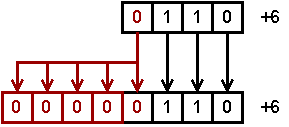
\includegraphics[width=.34\textwidth]{extend_4t8_sp}\hspace{8mm}
  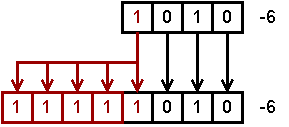
\includegraphics[width=.34\textwidth]{extend_4t8_sn}\\[1mm]
  {\small Positive \hspace{.28\textwidth} Negative}
  \begin{itemize}
    \item To widen a two's-complement number, \alert{copy the sign bit} into the new high-order bits.
    \item The value is unchanged. (Unsigned numbers are padded with 0s instead.)
  \end{itemize}
\end{frame}

\begin{frame}{Comparing the Systems (4 bits)}
  \begin{columns}[c]
  \begin{column}{.5\textwidth}
    \centering\scriptsize\striped
    \begin{tabular}{@{}ccccc@{}}
      \toprule
      \textbf{Bits} & \textbf{Unsig.} & \textbf{SM} & \textbf{1C} & \textbf{2C} \\
      \midrule
      1111 & 15 & $-7$ & $-0$ & $-1$ \\
      1110 & 14 & $-6$ & $-1$ & $-2$ \\
      1101 & 13 & $-5$ & $-2$ & $-3$ \\
      1100 & 12 & $-4$ & $-3$ & $-4$ \\
      1011 & 11 & $-3$ & $-4$ & $-5$ \\
      1010 & 10 & $-2$ & $-5$ & $-6$ \\
      1001 & 9 & $-1$ & $-6$ & $-7$ \\
      1000 & 8 & $-0$ & $-7$ & $-8$ \\
      0000--0111 & 0--7 & 0--7 & 0--7 & 0--7 \\
      \bottomrule
    \end{tabular}
  \end{column}
  \begin{column}{.48\textwidth}
    \centering\small\striped
    \begin{tabular}{@{}lccc@{}}
      \toprule
      & \textbf{SM} & \textbf{1C} & \textbf{2C} \\
      \midrule
      Smallest & $-(2^{n-1}-1)$ & $-(2^{n-1}-1)$ & $-2^{n-1}$ \\
      Largest & $2^{n-1}-1$ & $2^{n-1}-1$ & $2^{n-1}-1$ \\
      Zeros & 2 & 2 & \alert{1} \\
      \bottomrule
    \end{tabular}
    \vspace{3mm}
    \begin{itemize}\small
      \item MSB = 0: every system gives the same value.
      \item A byte: unsigned 0 to 255; two's complement $-128$ to $+127$.
    \end{itemize}
  \end{column}
  \end{columns}
\end{frame}

\begin{frame}{Back to the Opening Question}
  \begin{block}{Range of 4-bit two's complement}
    \small With $n = 4$ the range is $-2^{n-1}$ to $+(2^{n-1}-1)$: $-8$ to $+7$, sixteen values in all.\\[1mm]
    Zero uses one pattern ($0000$) and the sign bit splits the remaining 15 patterns unevenly: seven positive ($0001$ to $0111$) and eight negative ($1000$ to $1111$). The extra one is $1000 = -8$, which has no positive counterpart in 4 bits.
  \end{block}
\end{frame}

\begin{frame}{Preview: Addition and Overflow (Chapter 9)}
  \begin{itemize}\small
    \item One $n$-bit adder adds signed and unsigned numbers alike; subtract by adding the negation.
    \item \alert{Overflow}: the true result does not fit in $n$ bits. It happens only when adding two numbers of the \emph{same sign} and the result's sign differs.
    \item Equivalent test: carry \emph{into} the sign bit $\ne$ carry \emph{out of} it.
  \end{itemize}
  \begin{columns}[t]
  \begin{column}{.33\textwidth}
    \begin{block}{$5 + 4$}
      \small $0101 + 0100 = 1001$\\
      reads as $-7$: \alert{overflow}
    \end{block}
  \end{column}
  \begin{column}{.33\textwidth}
    \begin{block}{$5 + 5$}
      \small $0101 + 0101 = 1010$\\
      reads as $-6$: \alert{overflow}
    \end{block}
  \end{column}
  \begin{column}{.33\textwidth}
    \begin{block}{$-2 + -3$}
      \small $1110 + 1101 = 1\,1011$\\
      $= -5$, carry-out 1 but \alert{no} overflow
    \end{block}
  \end{column}
  \end{columns}
  \vspace{2mm}
  {\small A result outside the range $-8$ to $+7$ (4 bits) cannot be represented, so the hardware must raise an \alert{overflow flag}. Chapter 9 covers addition in detail.}
\end{frame}

%===============================================================================
\section{Real Numbers}
%===============================================================================

\begin{frame}{Representing Real Numbers}
  \begin{columns}[c]
  \begin{column}{.48\textwidth}
    \centering
    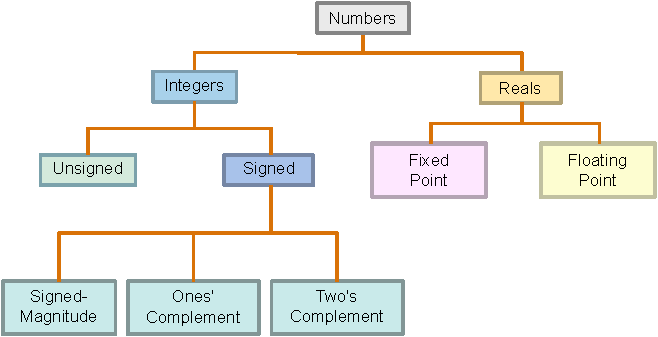
\includegraphics[width=\textwidth]{numbertypes}
  \end{column}
  \begin{column}{.5\textwidth}
    \small\striped
    \begin{tabular}{@{}lcR{.3\textwidth}@{}}
      \toprule
      \textbf{System} & \textbf{Format} & \textbf{Note} \\
      \midrule
      Rational & $\pm p/q$ & Difficult to work with \\
      Fixed-point & $\pm i.f$ & Low precision \\
      Floating-point & $\pm m\cdot b^e$ & Most common for reals \\
      \bottomrule
    \end{tabular}
    \vspace{2mm}
    \begin{itemize}\small
      \item No computer system can represent all real numbers.
      \item We cover fixed-point and floating-point.
    \end{itemize}
  \end{column}
  \end{columns}
\end{frame}

%===============================================================================
\section{Fixed-Point Numbers}
%===============================================================================

\begin{frame}{Fixed-Point Numbers}
  \begin{itemize}
    \item A fixed number of bits for the integer part and the fraction. The \alert{binary point} is \emph{not stored}; the designer remembers where it is.
  \end{itemize}
  \[ x = \frac{-b_{N-1}2^{N-1} + b_{N-2}2^{N-2} + \cdots + b_0 2^0}{2^f} \]
  \begin{block}{Example: $0101.1100_2$ (8 bits, $f = 4$)}
    \small $0 + 4 + 0 + 1 + 0.5 + 0.25 + 0 + 0 = 5.75_{10}$. Stored as $01011100_2$.
  \end{block}
\end{frame}

\begin{frame}{Q-Format}
  \begin{columns}[c]
  \begin{column}{.5\textwidth}
    \begin{itemize}\small\itemsep2pt
      \item Q$f$: 1 sign bit and $f$ fractional bits. Q7 = 8 bits; Q15 = 16 bits.
      \item Range $[-1,\ 1 - 2^{-f}]$. The value $+1$ cannot be represented.
      \item Common in DSP, embedded systems and TinyML: integer hardware does fractional maths.
    \end{itemize}
  \end{column}
  \begin{column}{.48\textwidth}
    \centering
    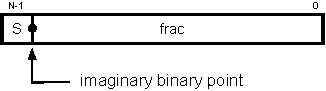
\includegraphics[width=\textwidth]{qformat}
  \end{column}
  \end{columns}
  \begin{block}{Q7 limits}
    \small Min $10000000 = -1.0$; max $01111111 = 0.9921875$; resolution $2^{-7} = 0.0078125$.
  \end{block}
\end{frame}

\begin{frame}{Example: 0.8 in Q7 and Q15}
  \begin{block}{$0.8_{10} = 0.110011001100\ldots_2$ (not exact)}
    \small
    \begin{itemize}\itemsep2pt
      \item Q7: $0.1100110_2 = 0.796875$; error about $0.39\%$.
      \item Q15: $0.110011001100110_2 = 0.79998779296875$; error about $0.0015\%$.
    \end{itemize}
  \end{block}
  \begin{itemize}
    \item More bits give better accuracy but more hardware cost and latency.
    \item Choose the \alert{minimum} precision that meets the quality requirement.
  \end{itemize}
\end{frame}

\begin{frame}{Q-Format Arithmetic}
  \begin{itemize}\small\itemsep2pt
    \item Q-format uses the \alert{same integer circuits}; only the interpretation differs.
    \item Adding two $m$-bit numbers gives an $(m+1)$-bit sum. Check the overflow flag.
    \item Multiplying $m$-bit by $n$-bit gives an $(m+n)$-bit product.
  \end{itemize}
  \centering
  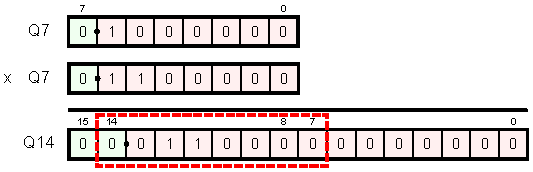
\includegraphics[height=.3\textheight]{q7mult_basic}\\[1mm]
  {\small $0.5 \times 0.75$: $01000000 \times 01100000 = 0001\,1000\,0000\,0000$ (two sign bits)}
  \begin{itemize}\small
    \item Systems keep one data width, so the product is cut back to Q7.
  \end{itemize}
\end{frame}

\begin{frame}{Truncation versus Rounding}
  \begin{columns}[c]
  \begin{column}{.5\textwidth}
    \centering
    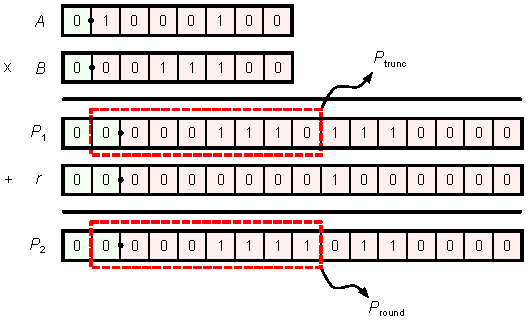
\includegraphics[width=\textwidth]{q7mult_round}
  \end{column}
  \begin{column}{.48\textwidth}
    \small
    \begin{itemize}\itemsep2pt
      \item Example: $0.53125 \times 0.21875$; exact $= 0.1162109375$.
      \item \alert{Truncation} drops low bits: $0.109375$, error $5.9\%$.
      \item \alert{Rounding}: add $r = 2^6$ first, then truncate: $0.1171875$, error $0.8\%$.
    \end{itemize}
  \end{column}
  \end{columns}
\end{frame}

%===============================================================================
\section{Floating-Point Numbers}
%===============================================================================

\begin{frame}{Floating-Point: Significand and Exponent}
  \begin{columns}[c]
  \begin{column}{.5\textwidth}
    \begin{itemize}\small\itemsep2pt
      \item $X = m \times b^e$: the radix point \alert{floats} as the exponent changes.
      \item Huge dynamic range, but costs more hardware and energy than fixed-point.
      \item Normalized binary form has a leading 1 before the point, e.g.
    \end{itemize}
    \[ 5.25_{10} = 101.01_2 = 1.0101_2 \times 2^2 \]
    \small IEEE 754 does not store the leading 1: the \alert{implicit 1} gives one extra bit of precision.
  \end{column}
  \begin{column}{.48\textwidth}
    \centering
    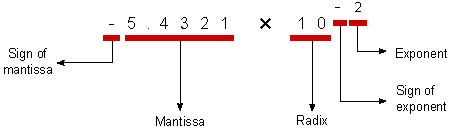
\includegraphics[width=\textwidth]{fpparts}
  \end{column}
  \end{columns}
\end{frame}

\begin{frame}{IEEE 754 Single Precision (FP32)}
  \centering
  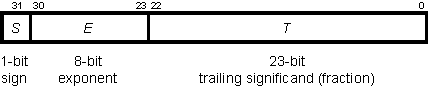
\includegraphics[width=.7\textwidth]{ieee754single}
  \begin{block}{Normal numbers ($1 \le E \le 254$)}
    \[ X = (-1)^S \times \left(1 + \frac{T}{2^{23}}\right) \times 2^{E-127} \]
  \end{block}
  \begin{itemize}\small\itemsep1pt
    \item $S$: sign, 1 bit. $E$: exponent, 8 bits, \alert{bias 127}. $T$: trailing significand, 23 bits.
    \item 24-bit precision, about 7 significant decimal digits.
  \end{itemize}
\end{frame}

\begin{frame}{FP32 Examples}
  \begin{columns}[t]
  \begin{column}{.5\textwidth}
    \begin{block}{Decode \texttt{1 10000001 11000...0}}
      \small
      $S = 1$, $E = 129$, $m = 1.11_2 = 1.75$\\
      $X = -1.75 \times 2^{129-127} = -7$
    \end{block}
  \end{column}
  \begin{column}{.48\textwidth}
    \begin{block}{Encode $17.0$}
      \small
      $17 = 10001_2 = 1.0001_2 \times 2^4$\\
      $S = 0$, $E = 127 + 4 = 131 = 10000011_2$\\
      \texttt{0 10000011 0001000...0}
    \end{block}
  \end{column}
  \end{columns}
\end{frame}

\begin{frame}{Special Values and Subnormals}
  \begin{columns}[t]
  \begin{column}{.55\textwidth}
    \centering\scriptsize\striped
    \begin{tabular}{@{}lccl@{}}
      \toprule
      \textbf{Value} & $E$ & $T$ & \textbf{Hex} \\
      \midrule
      $+0$ & 0 & 0 & 0x00000000 \\
      $-0$ & 0 & 0 & 0x80000000 \\
      $1.0$ & 127 & 0 & 0x3F800000 \\
      $+\infty$ & 255 & 0 & 0x7F800000 \\
      $-\infty$ & 255 & 0 & 0xFF800000 \\
      NaN & 255 & $\ne 0$ & 0x7FFFFFFF \\
      Largest normal & 254 & all 1s & 0x7F7FFFFF \\
      Smallest normal & 1 & 0 & 0x00800000 \\
      \bottomrule
    \end{tabular}
  \end{column}
  \begin{column}{.43\textwidth}
    \begin{itemize}\small\itemsep2pt
      \item \alert{Subnormal}: $E = 0$, $T \ne 0$; leading bit 0; fills the gap between 0 and $2^{-126}$ (gradual underflow).
      \item Exceptions: invalid, divide by zero, overflow, underflow, inexact.
    \end{itemize}
  \end{column}
  \end{columns}
\end{frame}

\begin{frame}{Other Floating-Point Formats}
  \centering\small\striped
  \begin{tabular}{@{}lcccc@{}}
    \toprule
    \textbf{Format} & \textbf{Bytes} & \textbf{Exponent bits} & \textbf{Fraction bits} & \textbf{Precision (bits)} \\
    \midrule
    FP16 (half) & 2 & 5 & 10 & 11 \\
    FP32 (single) & 4 & 8 & 23 & 24 \\
    FP64 (double) & 8 & 11 & 52 & 53 \\
    FP128 (quad) & 16 & 15 & 112 & 113 \\
    BF16 (bfloat16) & 2 & 8 & 7 & 8 \\
    FP8 E4M3 & 1 & 4 & 3 & 4 \\
    FP8 E5M2 & 1 & 5 & 2 & 3 \\
    \bottomrule
  \end{tabular}
  \begin{itemize}\small
    \item BF16 and FP8 are used in machine learning: same range as FP32 (BF16) or a range/precision trade-off (FP8).
  \end{itemize}
\end{frame}

%===============================================================================
\section{Summary}
%===============================================================================

\begin{frame}{Summary}
  \begin{itemize}\itemsep3pt\small
    \item \alert{Two's complement} dominates: a single representation of zero and a simple positional formula with sign-bit weight $-2^{n-1}$.
    \item Negate by inverting every bit and adding 1.
    \item Fixed-point trades range for simplicity; floating-point trades hardware for dynamic range.
    \item IEEE 754 single precision: sign (1), biased exponent (8), trailing significand (23).
  \end{itemize}
  \begin{block}{Looking ahead}
    Numbers in, numbers out. Chapter 4 introduces the logic gates that carry out every operation on those numbers.
  \end{block}
\end{frame}

\begin{frame}{One Last Thing}
  \centering
  
\includegraphics[height=.62\textheight]{codestoon03}\\[2mm]
  {\small Hint: read the 10 as a binary number.}
\end{frame}

\end{document}
